\chapter{Первое знакомство с Simics}\label{chap:lab01}

\section{Цель занятия}

Ознакомиться с базовыми операциями, которые можно выполнять в рабочем окружении (\abbr workspace) симулятора Simics.

\begin{itemize*}
    \item Запуск симулятора. Элементы его интерфейса.
    \item Сценарии работы. Гостевые системы. 
    \item Процесс загрузки гостевой операционной системы внутри симулятора.
    \item Базовые операции: остановка модели, сохранение и восстановление симуляции с диска и на диск.
\end{itemize*}

\section{Запуск симулятора Simics. Элементы интерфейса}

% Wind River\textregistered\ Simics~\cite{getting-started} --- это быстрый, функционально точный полноплатформенный симулятор. Simics позволяет создать виртуальное окружение, в котором любая электронная система, начиная с одной платы и заканчивая целыми многопроцессорными и многоядерными системами, может быть определена, разработана и запущена.

Для запуска Simics на физическом \textit{хозяйском} компьютере архитектуры IA-32 должны быть установлены следующие программы.

\begin{itemize*}
\item Вариант операционной системы GNU/Linux. Simics может работать практически во всех современных дистрибутивах, включая Debian, Ubuntu, Fedora, OpenSUSE и др. Настоятельно рекомендуются 64-битные варианты ОС.
\item Графическая оболочка, любая из поддерживаемых выбранным дистрибутивом: KDE, Gnome, Fluxbox и др. Несмотря на то, что Simics может работать из чистой командной строки, далее всюду в тексте книги будет подразумеваться, что работа ведётся в графическом режиме.
\item Собственно копия Simics. По-умолчанию программа устанавливается в подкаталог \texttt{/opt/simics/simics-4.6}, который будет использоваться всюду в тексте.
\end{itemize*}

Подробнее об аппаратных требованиях к используемым компьютерам сказано в~\cite{installation}. Особенности централизованной установки Simics в компьютерном классе описаны в приложении~\ref{chap:installation-notes}.

\subsection{Создание Simics workspace}

Одна инсталляция Simics может быть использована совместно множеством пользователей; по этой причине её файлы должны оставаться неизменными. Рабочее окружение (\abbr <<workspace>>\footnote{Начиная с Simics версии 4.8 название workspace было сменено на project, однако мы будем использовать традиционную терминологию.}) --- это персональная <<копия>> общей установки, в которой Simics хранит ваши собственные настройки симуляционной среды, сценарии для конфигурации гостевых систем, двоичный и исходный код моделей и прочие данные. Каждый пользователь может иметь несколько независимых workspace, все они могут использоваться одновременно и независимо друг от друга и содержать различные окружения.

\subsubsection{Создание workspace}

Для создания нового workspace необходимо выполнить следующую последовательность действий.

\begin{enumerate*}
    \item Создайте директорию, в которой будет находиться новый workspace (рекомендуется использовать локации внутри домашней директории \texttt{\$HOME}) и перейдите в неё:

\begin{lstlisting}
$ mkdir <folder_name>
$ cd <folder_name>
\end{lstlisting}
    \item Вызовите программу workspace-setup из инсталляции Simics. Учтите, что путь к инсталляции и версия Simics может отличаться.
\begin{lstlisting}
$ /opt/simics/simics-4.6/simics-4.6.32/bin/workspace-setup
Workspace created successfully
\end{lstlisting}
\end{enumerate*}

Новый workspace создан! Текущая директория теперь содержит несколько файлов и поддиректорий:
\begin{lstlisting}
$ ls -1
bin
compiler.mk
config.mk
doc-cache
GNUmakefile
modules
simics
simics-gui
targets
\end{lstlisting}


\subsection{Запуск Simics}

После создания workspace вы можете начинать работу с Simics. Запустить симулятор вы можете с помощью команды:

\begin{lstlisting}
./simics
\end{lstlisting}

Должно открыться окно управления \textbf{Simics Control}\footnote{Последние версии Simics используют в качестве базового графического окружения среду Eclipse~\cite{eclipse}. Поддержка предыдущего, классического интерфейса была сохранена в полной мере. В этой книге мы всюду будем использовать только его.} (рис.~\ref{fig:simics-control}). Оно включает в себя иконки панели инструментов и меню, позволяющее контролировать состояния симулятора и текущей гостевой системы. Для выполнения данных лабораторных работ нам понадобится дополнительное окно с командной строкой \textbf{Simics Command Line} (рис.~\ref{fig:simics-command-line}). Выберите \textbf{Tools $\to$ Command Line Window} для того, чтобы открыть его.

\begin{figure}[ht]
    \centering
    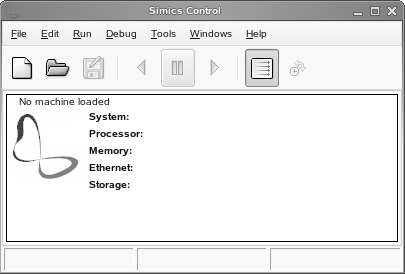
\includegraphics[width=0.6\textwidth]{./simics-control.png}
    \caption{Окно Simics Control}
    \label{fig:simics-control}
\end{figure}

\textbf{Simics Command Line} позволяет вам управлять симуляцией с помощью ввода текстовых команд. Во время своей работы Simics будет выводить в него диагностическую информацию: события симулятора и моделей, сообщения об ошибках и прочее. Всё, что можно сделать с помощью окна \textbf{Simics Control}, вы также можете сделать и с помощью командной строки. Большинство действий в дальнейшем будет производиться именно в ней.

\begin{figure}[ht]
    \centering
    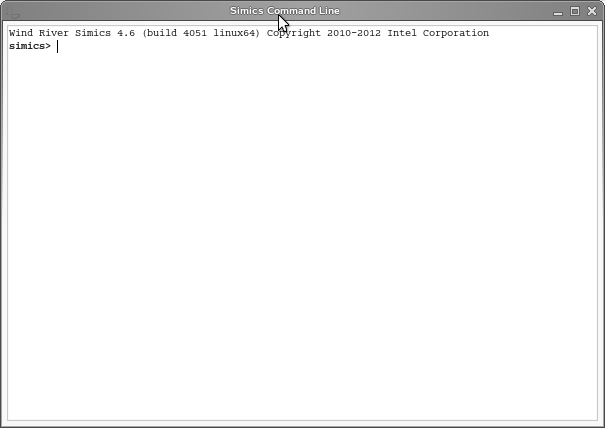
\includegraphics[width=0.6\textwidth]{./simics-command-line.png}
    \caption{Командная строка Simcs}
    \label{fig:simics-command-line}
\end{figure}

В данной главе в качестве моделируемой --- \textit{гостевой} --- используется вычислительная платформа, основанная на процессоре Intel\textsuperscript{\textregistered} Core\textsuperscript{\texttrademark} i7. GNU/Linux используется в качестве операционной системы. В качестве системной среды пользователя выступает пакет под названием BusyBox~\cite{BusyBox}, часто используемый во встраиваемых (\abbr embedded) системах.

Для загрузки конфигурации модели воспользуйтесь окном \textbf{Simics Command Line} и введите команду:

\begin{lstlisting}
simics> run-command-file targets/x86-x58-ich10/viper-firststeps.simics
\end{lstlisting}

То же самое можно было сделать с помощью окна \textbf{Simics Control}, выбрав \textbf{File $\to$ New session from script} и открыв файл \texttt{viper-firststeps.simics}, лежащий в директории \texttt{x86-x58-ich10}.

\paragraph{Автодополнение команд.} Если нажать несколько раз клавишу \textbf{Tab} при неполностью набранной строке команд, Simics автоматически дополнит её или предложит допустимые варианты для её завершения. Используйте это полезное свойство для ускорения набора и изучения списка понимаемых системой команд.

Спустя некоторое время окно \textbf{Simics Control} покажет суммарную информацию о симулируемой системе (рис.~\ref{fig:viper-control}): тип процессора, объём памяти, диска. Также должно открыться новое окно \textbf{Serial Console on viper.mb.sb.com[0]} (рис.~\ref{fig:viper-serial-console}).

\begin{figure}[ht]
    \centering
    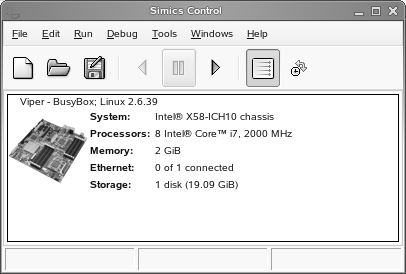
\includegraphics[width=0.6\textwidth]{./viper-control.png}
    \caption{Окно Simics Control после загрузки модели}
    \label{fig:viper-control}
\end{figure}

\begin{figure}[ht]
    \centering
    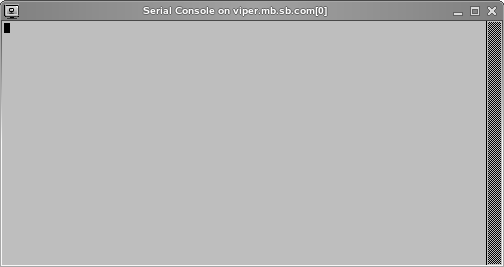
\includegraphics[width=0.6\textwidth]{./viper-serial-console.png}
    \caption[Окно Serial Console]{Окно \textbf{Serial Console on viper.mb.sb.com[0]}}
    \label{fig:viper-serial-console}
\end{figure}

Это новое окно является частью симуляции. Оно соединено с последовательным портом моделируемой материнской платы. Вывод сообщений гостевого ПО будет отображаться в нём. Кроме того, через него вы сможете взаимодействовать с моделируемым программным обеспечением, тогда как \textbf{Simics Command Line} используется для управления симуляцией.

\subsection{Запуск моделирования}

Теперь Simics ожидает ваших команд, вводимых через панель инструментов или через командную строку. Вы можете запустить симуляцию с помощью нажатия кнопки $\triangleright$ \textbf{Run Forward} на панели инструментов или ввода команды \texttt{continue} в командной строке.

Рассмотрим следующий пример:

\begin{lstlisting}
simics> continue
\end{lstlisting}

Для паузы симуляции в любой момент наберите команду \texttt{stop}.

\begin{lstlisting}
running> stop
[viper.mb.cpu0.core[0][0]] cs:0xffffffff8100944d p:0x00100944d  MWait state
simics>
\end{lstlisting}

После запуска симуляции виртуальное время (указываемое в нижней части \textbf{Simics Control}) начинает увеличиваться, инструкции гостевого процессора исполняются, и сообщения от программного обеспечения выводятся в окно консоли. Если вы позволите модели поработать некоторое время, то увидите сообщения от загрузки гостевой ОС в окне \textbf{Serial Console on viper.mb.sb.com[0]} (рис.~\ref{fig:booted-linux}). Симуляция может быть остановлена с помощью команды \texttt{stop} или нажатия \textbf{Stop} на панели инструментов.

\begin{figure}
	\centering
	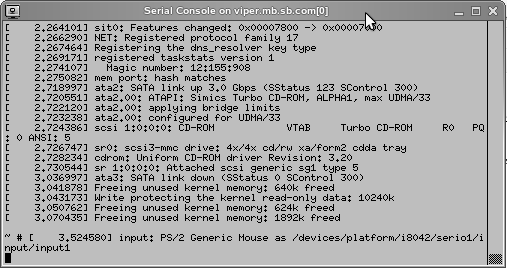
\includegraphics[width=0.6\textwidth]{./booted-linux.png}
	\caption{Загруженная гостевая операционная система Linux}
	\label{fig:booted-linux}
\end{figure}

После полной загрузки ОС в гостевой консоли будет выведено приглашение для логина пользователя:
\begin{lstlisting}
busybox login:
\end{lstlisting}

Введите в него \texttt{root}, нажмите \textbf{Enter}. Теперь гостевая операционная система загружена, и вы можете начать взаимодействовать с ней --- вводить инструкции в командной строке.

\paragraph{Получить листинг корневой директории.} Пример вывода команды \texttt{ls}:

\begin{lstlisting}
# ls /
bin      etc      host     linuxrc  root     sys
dev      home     init     proc     sbin     var
\end{lstlisting}

\paragraph{Увидеть информацию о моделируемом процессоре.} Пример содержимого псевдофайла \texttt{/proc/cpuinfo} гостевой системы:

\begin{lstlisting}
~ # cat /proc/cpuinfo                                                           
processor       : 0                                                             
vendor_id       : GenuineIntel                                                  
cpu family      : 6                                                             
model           : 26                                                            
model name      : Intel(R) Core(TM) i7 CPU     @ 2.00GHz               
stepping        : 8                                                             
cpu MHz         : 1999.991                                                      
cache size      : 8192 KB                                                       
fpu             : yes                                                           
fpu_exception   : yes                                                           
cpuid level     : 11                                                            
wp              : yes                                                           
flags           : fpu vme de pse tsc msr pae mce cx8 apic sep mtrr pge mca cmov pat pse36 clflush dts acpi mmx fxsr sse sse2 ss tm pbe syscall nx rdtscp lm constant_tsc up arch_perfmon pebs bts rep_good nopl xtopology nonstop_tsc aperf mperf pni dtes64 monitor ds_cpl vmx est tm2 ssse3 cx16 xtpr pdcm sse4_1 sse4_2 popcnt lahf_lm ida dts tpr_shadow ept
bogomips        : 3999.98                                                       
clflush size    : 64                                                            
cache_alignment : 64                                                            
address sizes   : 36 bits physical, 48 bits virtual                             
power management:                                                               
\end{lstlisting}

Для того чтобы закончить работу симулятора, необходимо выполнить команду \texttt{quit}. Более подробно о командах Simics рассказывается в последующих главах, а также в приложении~\ref{chap:append01}.

\section{Сохранение и восстановление состояния симуляции}

Так как в любой момент исполнения симуляции известны состояния всех моделируемых внутри неё устройств, имеется возможность записать их в постоянное хранилище, например, в файл. В дальнейшем эту точку сохранения (\abbr checkpoint) можно загрузить и продолжить симуляцию с той точки, в которой она была сохранена.

В Simics для создания точки сохранения используется команда \texttt{write-configuration <name>}.

\begin{itemize*}
    \item Запустите симуляцию. Позвольте ей исполняться в течение нескольких виртуальных секунд:
\begin{lstlisting}
$ ./simics targets/x86-x58-ich10/viper-firststeps.simics
simics> continue-seconds 3
simcis> write-configuration new-chkpt
\end{lstlisting}
    \item Завершите сессию симуляции с помощью команды \texttt{quit}.
    
    \item Проверьте, что в текущем workspace была создана новая директория с именем \texttt{new-chkpt}.
\begin{lstlisting}
$ ls -1
bin
compiler.mk
config.mk
doc-cache
GNUmakefile
modules
new-chkpt
simics
simics-gui
targets    
\end{lstlisting}
В ней сохранено состояние всей симуляции на момент выполнения команды сохранения.
    \item Запустите пустую сессию Simics, без загрузки каких-либо сценариев:
\begin{lstlisting}
$ ./simics
\end{lstlisting}

\item Загрузите точку сохранения с помощью команды \texttt{read-configuration}:
\begin{lstlisting}
simcis> read-configuration new-chkpt
\end{lstlisting}
В результате состояния симуляции будет эквивалентно тому, что она имела на момент создания точки.
\item Продолжите исполнение симуляции с помощью \texttt{continue} и убедитесь, что загрузка системы продолжается корректно.
\end{itemize*}



% \section{Задания}

% \begin{enumerate*}
    % \item Загрузить модель Viper с операционной системой BusyBox~\cite{BusyBox}. Для этого необходимо из вашего workspace выполнить команду
% \begin{lstlisting}
% ./simics targets/x86-x58-ich10/viper-busybox.simics
% \end{lstlisting}
    % \item Открыть окно \textbf{Simics Command Line} и запустить симуляцию.
    % \item Сравнить содержимое файла \texttt{/proc/cpuinfo} симулируемой и реальной машины.
    % \item Найти способы определения факта нахождения внутри симулятора (имена устройств будут выдавать факт виртуализации).
% \end{enumerate*}

\section{Задания и контрольные вопросы к главе}

\begin{enumerate*}
\item Определите все отличия в параметрах аппаратных средств гостевой и хозяйской систем, используемых в данной работе. Какие средства могут быть использованы для обнаружения различий?
\item Сравните скорость течения виртуального времени, сообщаемого симуляцией, и настоящего времени. Чем, по-вашему, вызваны наблюдаемые различия?
\item Попытайтесь удалить \emph{все} файлы внутри симуляции. Каким образом это действие скажется на хозяйской системе? Перезапустите симуляцию. Что произошло с удалёнными файлами?

\item Придумайте сценарии применения точек сохранения симуляции а практике разработки ПО и аппаратных средств с помощью симуляторов.

\end{enumerate*}

\iftoggle{webpaper}{
    \printbibliography[title={Список литературы к занятию}]
}{}


%%%%%%%%%%%%%%%%%%%%%%%%%%%%%%%%%%%%%%%% Legacy cluster.iscalare.mipt.ru notes %%%%%%%%%%%%%%%%%%%%%%%%%%%%%%%%%%%%%%%%%%%%%%%%%%%%%

% \subsection{Доступ на удалённую систему через SSH}\label{subsec:ssh}

% SSH (\abbr Secure SHell --- <<безопасная оболочка>>)~\cite{openssh} --- сетевой протокол прикладного уровня, позволяющий производить удаленное управление операционной системой и туннелирование TCP-соединений (например, для передачи файлов). SSH-клиенты и SSH-серверы доступны для большинства сетевых операционных систем.

% Ниже будут описаны способы использования SSH из-под операционных систем Linux и Windows.

% \subsubsection{Linux}

% Откройте терминал и наберите команду, заменив слово \texttt{user} на свой логин:

% \begin{lstlisting}
% $ ssh user@cluster.iscalare.mipt.ru
% \end{lstlisting}

% После этого система спросит у вас пароль. Введите его. Внимание! Вводимые символы не отображаются на экране. При удачном вводе пароля вы увидите сообщения приветствия командной строки (рис.~\ref{fig:ssh-login}).

% \subsubsection{Windows}

% Для того чтобы подключаться к удаленному серверу из системы Windows, необходимо воспользоваться SSH-клиентом, например, PuTTY~\cite{putty} (мы рекомендуем использовать именно его):

% \begin{enumerate*}
    % \item Запустите PuTTY.
    % \item В главном окне программы в поле \textbf{Host Name (or IP address)} введите строку \texttt{user@cluster.iscalare.mipt.ru}, заменив \texttt{user} на свой логин (рис.~\ref{fig:putty}).
    % \item Порт оставьте равным 22.
    % \item Сохраните сессию под некоторым именем, чтобы избежать необходимости повторного ввода в дальнейшем.
    % \item После открытия окна вам будет предложено ввести пароль. Введите его и нажмите \textbf{Enter}. Внимание: вводимые символы не отображаются на экране!
    % \item При удачном входе вы получите приглашение командной строки (рис.~\ref{fig:ssh-login}).
% \end{enumerate*}

% \begin{figure}[htb]
    % \centering
    % 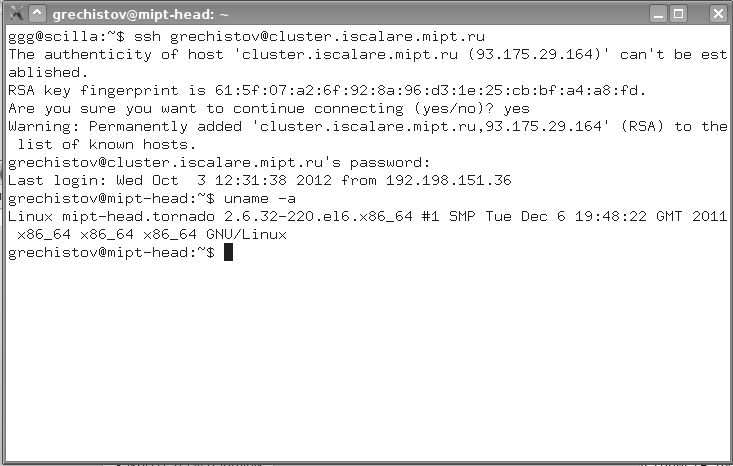
\includegraphics[width=0.6\textwidth]{./ssh-login}
    % \caption{Открытие сессии SSH}
    % \label{fig:ssh-login}
% \end{figure}

% \begin{figure}[htb]
    % \centering
    % 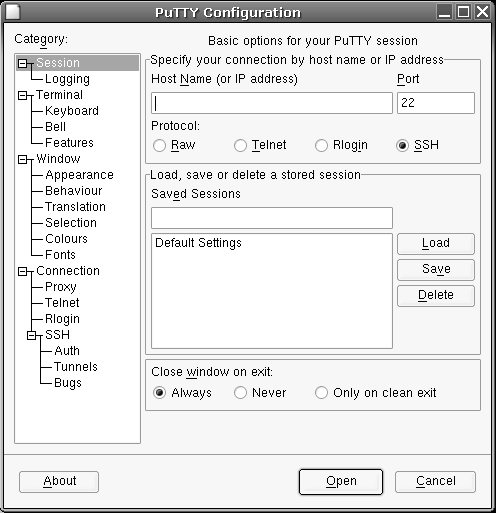
\includegraphics[width=0.6\textwidth]{./putty.png}
    % \caption{Окно PuTTY}
    % \label{fig:putty}
% \end{figure}

% \subsection{Создание VNC-сессии}

% VNC (\abbr Virtual Network Computing)~\cite{vnc} --- система удалённого доступа к рабочему столу компьютера, использующая протокол RFB (\abbr Remote Frame Buffer). VNC состоит из двух частей: клиента и сервера. Сервер — программа, предоставляющая доступ к экрану компьютера, на котором она запущена. Клиент (\abbr viewer) --- программа, получающая изображение экрана с сервера и взаимодействующая с ним по протоколу RFB. Управление осуществляется путём передачи нажатий клавиш на клавиатуре и движений мыши с одного компьютера на другой и ретрансляции содержимого экрана через компьютерную сеть. Система VNC платформонезависима: VNC-клиент, запущенный на одной операционной системе, может подключаться к VNC-серверу, работающему на любой другой ОС. Существуют реализации клиентской и серверной части практически для всех операционных систем, в том числе и для Java (включая мобильную платформу J2ME). К одному VNC-серверу одновременно могут подключаться множественные клиенты. Наиболее популярные способы использования VNC — удалённая техническая поддержка и доступ к рабочему компьютеру из дома.

% \subsubsection{Использование VNC для доступа к удаленному серверу}

% Для создани VNC-сессии необходимо выполнить следующую последовательность действий:

% \begin{enumerate*}
    % \item Зайдите на удалённый сервер, как описано в секции~\ref{subsec:ssh}.
    % \item Запустите команду для создания графического сервера с необходимым вам разрешением экрана:
% \begin{lstlisting}
% $ vncserver -geometry 1280x1024
% \end{lstlisting}
% Рекомендуется выбирать разрешение, равное или меньшее физического разрешения экрана вашей системы.
    % \item При необходимости (при первом запуске) задайте пароль (он не обязан совпадать с SSH-паролем). Пароль можно изменить впоследствии с помощью команды \texttt{vncpasswd}. Если вы забыли его, то удалить его можно, удалив файл \texttt{\$HOME/.vnc/passwd}.
    % \item Запомните номер сессии (число после двоеточия в выводе команды). Например, из вывода команды ниже видно, что только что созданный номер сессии равен 4.
% \begin{lstlisting}
% $ vncserver
% New 'mipt-head.tornado:4 (user)' desktop is mipt-head.tornado:4
% Starting applications specified in /home/user/.vnc/xstartup
% Log file is /home/user/.vnc/mipt-head.tornado:4.log
% \end{lstlisting}
% \textbf{Примечание.} Допускается иметь более одной VNC-сессии, при этом каждая будет иметь свой идентификатор (номер порта после двоеточия). Однако имейте в виду, что каждая из них потребляет небольшое количество общих системных ресурсов.
% Файл журнала соответствующей сессии, например \texttt{mipt-head.tornado:4.log}, полезен при анализе проблем при запуске, например, когда открываемый впоследствии графический экран пустой или VNC-сессия вообще не запустилась.
% \end{enumerate*}

% \subsubsection{Замечание о необходимости тунеллирования VNC}

% В настоящее время на \texttt{cluster.iscalare.mipt.ru} закрыты все внешние порты, кроме SSH (22). Поэтому для VNC-соединения, использующего порты в диапазоне 5901--5999, необходимо создавать т.н. \textbf{SSH-туннель}. Теоретически для локального конца туннеля можно выбирать любой порт (из непривилегированного диапазона 1001--65535), однако для избежания путаницы рекомендуется выбирать его равным номеру удалённого конца; в последующих примерах мы придерживаемся этого правила.

% \subsubsection{Отключение VNC-сессии}

% Обычно закрывать сессию VNC не требуется --- достаточно отключиться от неё. Затем можно возобновить работу, используя VNC-клиент. При необходимости уничтожение десктопа и всех запущенных приложений может быть выполнено командой

% \begin{lstlisting}
% $ vncserver -kill :4
% \end{lstlisting}

% Если необходимо уничтожить все свои VNC-сессии, используйте команду

% \begin{lstlisting}
% $ killall Xvnc
% \end{lstlisting}

% \subsubsection{Linux}

% Для начала нам необходимо установить VNC-клиент на наш рабочий компьютер (если он еще не установлен). Для установки клиента на персональную ЭВМ необходимо воспользоваться пакетным менеджером. Пример для Ubuntu/Debian:

% \begin{lstlisting}
% $ sudo apt-get install xtightvncviewer
% \end{lstlisting}

% Кроме того, допускается использовать любой клиент, поддерживающий протокол VNC: RealVNC, TighVNC, Remmina, Vinagre, Krdp\dots

% Затем используйте следующие опции \textbf{ssh} для создания туннеля (в примере ниже  --- для порта 5904, имени пользователя \texttt{user})

% \begin{lstlisting}
% $ ssh -L 5904:127.0.0.1:5904  -l user cluster.iscalare.mipt.ru
% \end{lstlisting}

% Если вы используете TightVNC, то для запуска VNC-сессии вам необходимо воспользоваться командой, указав после двоеточия номер вашей VNC-сессии (в данном примере номер VNC-сессии равен 4).

% \begin{lstlisting}
% $ vncviewer localhost:4
% \end{lstlisting}

% После этого система спросит у вас пароль. Введите его. Внимание! Вводимые символы не отображаются на экране. При удачном вводе пароля откроется окно VNC-сессии, готовое к работе. 

% \subsubsection{Windows}

% Для Windows мы рекомендуем использовать RealVNC. Инструкцию по установке и дополнительную информацию можно найти в~\cite{RealVNC}.

% Допускается использовать любой клиент, поддерживающий протокол VNC: RealVNC, TighVNC, UltraVNC\dots

% При открытии SSH из Putty дополнительно на складке Tunnels создаём проброс порта вашей VNC-сессии. В данном примере (рис.~\ref{fig:ssh-tunnel}) это экран VNC :4, что соответствует TCP-порту 5904.

% \begin{figure}[htb]
    % \centering
    % 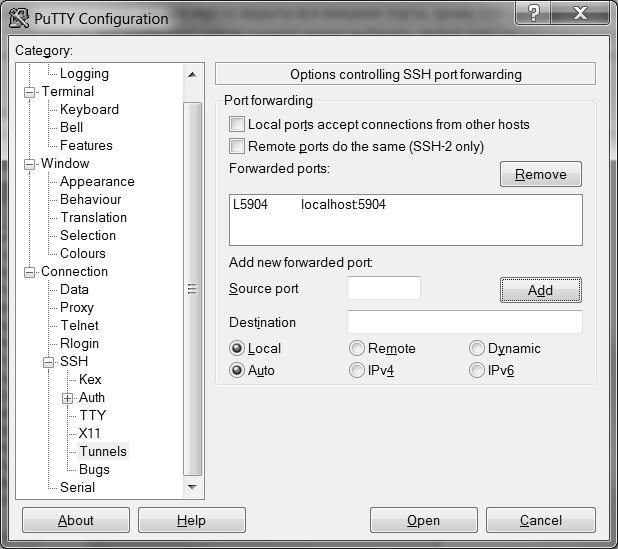
\includegraphics[width=0.6\textwidth]{./ssh-tunnel.png}
    % \caption{Создание ssh туннеля с помощью PuTTY}
    % \label{fig:ssh-tunnel}
% \end{figure}

% Для подключения к удаленному рабочему столу необходимо воспользоваться VNC-клиентом (в нашем примере это RealVNC). Выполните следующую последовательность действий:

% \begin{enumerate*}
    % \item Откройте VNC viewer.
    % \item В поле VNC Server укажите \textbf{localhost:4} (рис.~\ref{fig:realvnc}), заменив число 4 после двоеточия на номер вашей VNC-сессии.

% \begin{figure}[htb]
    % \centering
    % 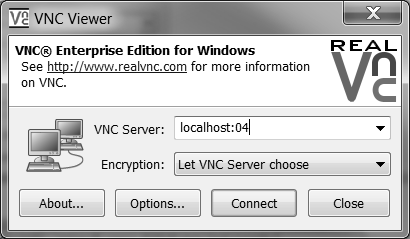
\includegraphics[width=0.5\textwidth]{./realvnc.png}
    % \caption{Окно RealVNC}
    % \label{fig:realvnc}
% \end{figure}

    % \item Нажмите \textbf{Connect}.
    % \item Система запросит ваш пароль от VNC-сессии. Введите его.
    % \item При удачном вводе пароля откроется окно VNC-сессии готовое к работе.
% \end{enumerate*}

% \subsection{Базовые команды Linux}

% В этой секции перечислены команды Linux, которые понадобятся для выполнения данной лабораторной работы:

% \begin{itemize*}
    % \item Команда \textbf{man} предназначена для формирования и  вывода справочной информации о команде \texttt{<command>}:
% \begin{lstlisting}
% $ man <command>
% \end{lstlisting}

    % \item Команда \texttt{ls} выводит информацию о \texttt{<file>} (по умолчанию выводится информация о текущей директории).
% \begin{lstlisting}
% $ ls <file>
% \end{lstlisting}

    % \item Команда \texttt{cd} меняет текущую рабочую директорию на \texttt{<directory>}.
% \begin{lstlisting}
% $ cd <directory>
% \end{lstlisting}

    % \item Команда \texttt{mkdir} создает директорию \texttt{<directory>} в текущей, если она до этого не существовала.
% \begin{lstlisting}
% $ mkdir <directory>
% \end{lstlisting}

    % \item Команда \texttt{cat} направляет \texttt{<file>} на стандартный вывод. Чаще всего это означает распечатывание его содержимого на экране.
% \begin{lstlisting}
% $ cat <file>
% \end{lstlisting}

    % \item Команда \texttt{lspci} показывает список всех PCI-устройств.
    % \item Команда \texttt{mount [node] <folder>} монтирует файловую систему; вызванная без аргументов, она перечисляет уже смонтированные системы.
    % \item Команда \texttt{umount <folder>} предназначена для отмонтирования файловой системы.
% \end{itemize*}

% Больше информации о командах Linux вы можете найти в мануалах, воспользовавшись командой \textbf{man}, описанной выше.
